\documentclass[9pt,letterpaper]{extarticle}

\usepackage[left=0.5in,right=0.5in,top=0.58in,bottom=0.5in,headheight=11pt,headsep=6pt,footskip=14pt]{geometry}
\usepackage{amsmath}
\usepackage{booktabs}
\usepackage{array}
\usepackage{tabularx}
\usepackage{graphicx}
\usepackage{xcolor}
\usepackage{caption}
\usepackage{enumitem}
\usepackage{needspace}
\usepackage{fancyhdr}
\usepackage{lastpage}
\usepackage{microtype}
\usepackage{hyperref}

\graphicspath{{../figures/}}

\definecolor{navy}{RGB}{0,48,87}
\definecolor{slate}{RGB}{84,88,90}
\hypersetup{colorlinks=true, linkcolor=navy, urlcolor=navy,
  pdftitle={Corporate Loan Pricing with Machine Learning}, pdfauthor={Thanh Vy Vo}}

\setlist{noitemsep, topsep=1pt, parsep=0pt, partopsep=0pt, leftmargin=13pt}
\setlength{\parskip}{2pt}
\emergencystretch=2em
\setlength{\parindent}{0pt}
\renewcommand{\arraystretch}{1.08}
\captionsetup{font=footnotesize, labelfont={bf,color=navy}, labelsep=period, skip=3pt, width=\textwidth}

\makeatletter
\renewcommand\section{\@startsection{section}{1}{\z@}{6pt plus 2pt minus 1pt}{3pt plus 1pt}%
  {\normalfont\large\bfseries\color{navy}}}
\renewcommand\subsection{\@startsection{subsection}{2}{\z@}{4pt plus 1pt minus 1pt}{2pt plus 1pt}%
  {\normalfont\normalsize\bfseries\color{navy}}}
\makeatother

\pagestyle{fancy}
\fancyhf{}
\lhead{\footnotesize\textcolor{slate}{\textbf{Corporate Loan Pricing with Machine Learning}}}
\rhead{\footnotesize\textcolor{slate}{\textbf{Thanh Vy Vo}}}
\lfoot{\footnotesize\textcolor{slate}{Data: linked DealScan, Compustat, CRSP and FRED extract, 1996-2019}}
\rfoot{\footnotesize\textcolor{slate}{Page \thepage\ of \pageref{LastPage}}}
\renewcommand{\headrulewidth}{0.4pt}
\renewcommand{\footrulewidth}{0.4pt}

\begin{document}

% ======================================================================
% PAGE 1: main finding, performance table, design
% ======================================================================
\begin{center}
  {\Large\bfseries\color{navy} Corporate Loan Pricing with Machine Learning}\\[2pt]
  {\normalsize Thanh Vy Vo}
\end{center}
\vspace{-4pt}

\section*{Main finding}
The validation-selected preferred model is \textbf{Gradient boosting (depth 3, min leaf 20)}. It has the lowest validation RMSE (70.9~bps; MAE 43.8~bps) among OLS, Ridge and gradient boosting, a choice fixed before any test target was read, and it was then refit on the training plus validation loans (6,326 facilities) and scored on 1,279 later loans. It is substantially more accurate than the constant benchmark on the test sample (RMSE 60.4 vs 74.7~bps, 19.2\% lower; the borrower-clustered bootstrap 95\% interval for the difference, [$-$19.1, $-$9.6]~bps, excludes zero); it has $R^2_{\mathrm{OOS}}$ = 0.347, i.e. 34.7\% lower test squared error than the train+validation mean benchmark, of which 0.054 from a smaller level error and 0.293 from smaller errors around the mean.

\begin{itemize}
  \item \textbf{Validation margin.} Against the runner-up, the preferred model and OLS are about equally accurate on the validation sample (RMSE 70.9 vs 71.9~bps, a difference of 1.4\%). The choice therefore follows the pre-set rule of the lowest validation RMSE; the margin of 1.0~bps (1.4\%) is small and should not be read as a robust advantage.
  \item \textbf{Test ranking.} By test RMSE the order is Ridge and OLS (54.4~bps each, about equally accurate), then Gradient boosting (60.4~bps); the preferred model is substantially less accurate than Ridge on the test sample (RMSE 60.4 vs 54.4~bps, 11.1\% higher; the borrower-clustered bootstrap 95\% interval for the difference, [4.0, 7.9]~bps, excludes zero). The validation-selected model is kept as the preferred model, as required: choices were frozen before the test sample was scored, and one chronological split can rank models differently in other periods.
  \item \textbf{Information blocks.} The loan and industry block carries the most predictive information: shuffling its columns jointly raises the preferred model's validation RMSE by 17.5~bps, against 9.9~bps for the borrower financials block, 1.4~bps for the market history block, and 0.2~bps for the macroeconomy block. The nested Ridge comparison is consistent with this but order-dependent (the first block to enter is credited with information it shares with later ones). On validation, Ridge on the loan block alone has a clearly lower RMSE than the constant benchmark (RMSE 75.5 vs 95.1~bps; the bootstrap interval excludes zero); adding borrower financials to the loan and industry block goes with a clearly lower RMSE (72.3 vs 75.5~bps), and the borrower-clustered interval excludes zero; and adding market history and macroeconomic variables to the first two blocks leaves the RMSE (71.9 vs 72.3~bps) about equal (within 2\%). The RMSE gains are 19.6, 3.2 and 0.4~bps, respectively. The nested comparison cannot separate market history from the macroeconomy, and it uses Ridge fits rather than the preferred model. These are predictive comparisons only.
  \item \textbf{Key limitation.} This is a retrospective pricing exercise on one chronological split (three validation years, two test years) of a selected linked sample, not a live underwriting backtest. Most test borrowers (89.5\%) had already appeared in the training or validation data, so results describe later loans to the observed borrower population, not new firms.
\end{itemize}

\begin{center}
\small
\begin{tabular}{@{}lrrrrr@{}}
\toprule
\textbf{Model} & \textbf{Valid.\ RMSE} & \textbf{Valid.\ MAE} & \textbf{Test RMSE} & \textbf{Test MAE} & \textbf{Test $R^2_{\mathrm{OOS}}$} \\
\midrule
Constant (fitting-sample mean) & 95.1 & 71.1 & 74.7 & 62.2 & 0.000 \\
OLS & 71.9 & 47.5 & 54.4 & 40.6 & 0.471 \\
Ridge ($\alpha$ = 0.01) & 71.9 & 47.5 & 54.4 & 40.6 & 0.471 \\
Gradient boosting (depth 3, min leaf 20)$^{\dagger}$ & 70.9 & 43.8 & 60.4 & 46.5 & 0.347 \\
\midrule
\emph{Ridge, log target ($\alpha$ = 10; supplementary)} & 70.2 & 44.9 & 51.0 & 34.9 & 0.534 \\
\bottomrule
\end{tabular}
\par\vspace{2pt}
\captionof{table}{Model performance in basis points (bps; 100 bps = 1 percentage point). The target is the DealScan all-in drawn spread, which includes annual fees and is not the total interest rate. Validation columns: models fitted on training loans, 1996-2014 (4,157 facilities), scored on validation loans, 2015-2017 (2,169 facilities); the Ridge penalty and boosting settings shown were chosen by validation RMSE. Test columns: the same specifications refit on training plus validation loans (6,326 facilities) and scored once on test loans, 2018-2019 (1,279 facilities). $R^2_{\mathrm{OOS}} = 1 - \sum_{i\in\mathrm{test}}(y_i-\hat y_i)^2 \,/\, \sum_{i\in\mathrm{test}}(y_i-\bar y_{\mathrm{train+val}})^2$ is measured against the train+validation mean spread, not the test mean; a negative value means worse than that benchmark, and it is not the usual $R^2$. $^{\dagger}$ Validation-selected preferred model. The italic row is a supplementary log-target model and is not eligible for selection.}
\end{center}

\needspace{6\baselineskip}
\section*{Design}
Facilities are split by the supplied labels into training (1996-2014, 4,157), validation (2015-2017, 2,169) and test (2018-2019, 1,279) loans; the data are never re-split at random. The target is \texttt{spread\_bps} and only the 20 supplied predictors (loan and industry, borrower financials, market history, macroeconomy) are used. The timing audit holds for every facility: accounting statements are used from six months after the period end (an assumed availability rule, not a filing date) and are 6 to 18 months old at origination; market features use the 12 months ending before the origination month; macroeconomic features use a reference month two months before origination. All preprocessing is fitted on the fitting sample only (training loans during selection, training plus validation loans at the final refit): 8 ratio and market columns are capped at the fitting-sample 1st and 99th percentiles, missing numeric values get median imputation plus missingness indicators, categories with fewer than 20 fitting facilities and unseen categories share one pooled column (a feature with no rare levels sends an unseen category to its reference level), and OLS and Ridge use standardized numeric inputs. Ridge tries 8 penalties and boosting 6 depth and minimum-leaf settings (300 trees, learning rate 0.05), all chosen by validation RMSE.

% ======================================================================
% PAGE 2: data and sample
% ======================================================================
\needspace{5\baselineskip}
\section*{Data and sample}
\begin{itemize}
  \item \textbf{Sample.} 7,605 facilities in 6,972 packages and 3,864 borrowers, originated 2 January 1996 to 30 December 2019. Facility identifiers are unique, the three splits are chronologically separated (all training loans precede all validation loans, which precede all test loans), and no deal package appears in more than one split.
  \item \textbf{Repeated borrowers.} Most of the 885 test borrowers (792, 89.5\%) had already appeared in the training or validation data, so results describe later loans to the observed borrower population, not new firms. They account for 1,163 test facilities (90.9\%).
  \item \textbf{Selected sample and coverage.} The data are a selected linked sample (DealScan facilities linked to Compustat and CRSP, in U.S. dollars, syndicated in the USA), not the universe of corporate loans. Facilities per year jump from 118 in 2012 to 828 in 2013 (7.02 times as many). This is a change in the coverage of the selected linked sample (the reason is not documented), not evidence about aggregate lending volume. Secured status is unknown for 24.5\% of the training loans (1996-2014) and 43.3\% of the test loans (2018-2019), so the test loans differ in composition from the training loans.
  \item \textbf{Missing features.} Blank cells mean unavailable information, not zero, and no loans are dropped. The largest gaps are \mbox{\texttt{return\_12m}} and \mbox{\texttt{volatility\_12m}} (31.16\%), \mbox{\texttt{current\_ratio}} (19.45\%), \mbox{\texttt{interest\_coverage}} (14.40\%), and \mbox{\texttt{operating\_income\_assets}} (8.15\%); every other predictor is missing for at most 8.01\%. By construction, market history is missing when the security link is ambiguous or the 12-month return history is incomplete; accounting ratios are missing when no eligible statement is matched (116 facilities) or when a component is missing or the denominator is not positive, which accounts for most of the 1,479 missing \mbox{\texttt{current\_ratio}} values; and 12 maturities are missing (by construction, nonpositive maturities are set to missing). The supplied CRSP extract starts in 1996 and the return window needs the 12 months before origination, so market history is available for 0.0\% of the 188 facilities originated in 1996 against 73.8\% in 1997. These gaps follow the construction rules, so missingness is not random.
  \item \textbf{Spreads in the training loans.} Training spreads (4,157 facilities) have a median of 175.0~bps, a mean of 196.5~bps and a standard deviation of 117.7~bps. All exploratory target summaries use training loans only.
  \item \textbf{Two economic relationships (training loans).} Secured status: training median spread 225.0~bps for secured loans (2,199) against 125.0~bps for unsecured (941; unknown status 137.0~bps), a gap of 100.0~bps. Two channels pull in opposite directions. Collateral lowers the lender's loss if the borrower defaults, which on its own would lower the spread; but lenders tend to ask riskier borrowers for collateral, so secured loans go to riskier borrowers on average, which goes with higher spreads. The training sample has secured loans priced higher, which is consistent with the second channel (collateral requested from riskier borrowers) outweighing the first; it does not measure the effect of collateral. Borrower size (\texttt{log\_assets}): the training median spread falls from 255.0~bps in the smallest-asset quintile to 125.0~bps in the largest (130.0~bps lower). Larger borrowers are usually viewed as lower credit risk, so the sign agrees with that expectation.
  \item \textbf{Other pre-specified summaries.} Top-quintile median spread against the bottom-quintile median: \mbox{\texttt{volatility\_\allowbreak{}12m}}, 150.0~bps above (rising across the quintiles); \mbox{\texttt{debt\_\allowbreak{}assets}}, 25.0~bps above (175.0, 150.0, 150.0, 175.0, 200.0~bps; not monotone); \mbox{\texttt{maturity\_\allowbreak{}months}}, 37.5~bps below (187.5, 225.0, 175.0, 150.0, 150.0~bps; not monotone). Of the training loans with a \texttt{maturity\_months} value, 61.7\% have a value shared with loans in another quintile; tied loans are assigned to quintiles in file order, which follows the origination date, so these quintiles partly sort loans by year.
\end{itemize}

\begin{center}
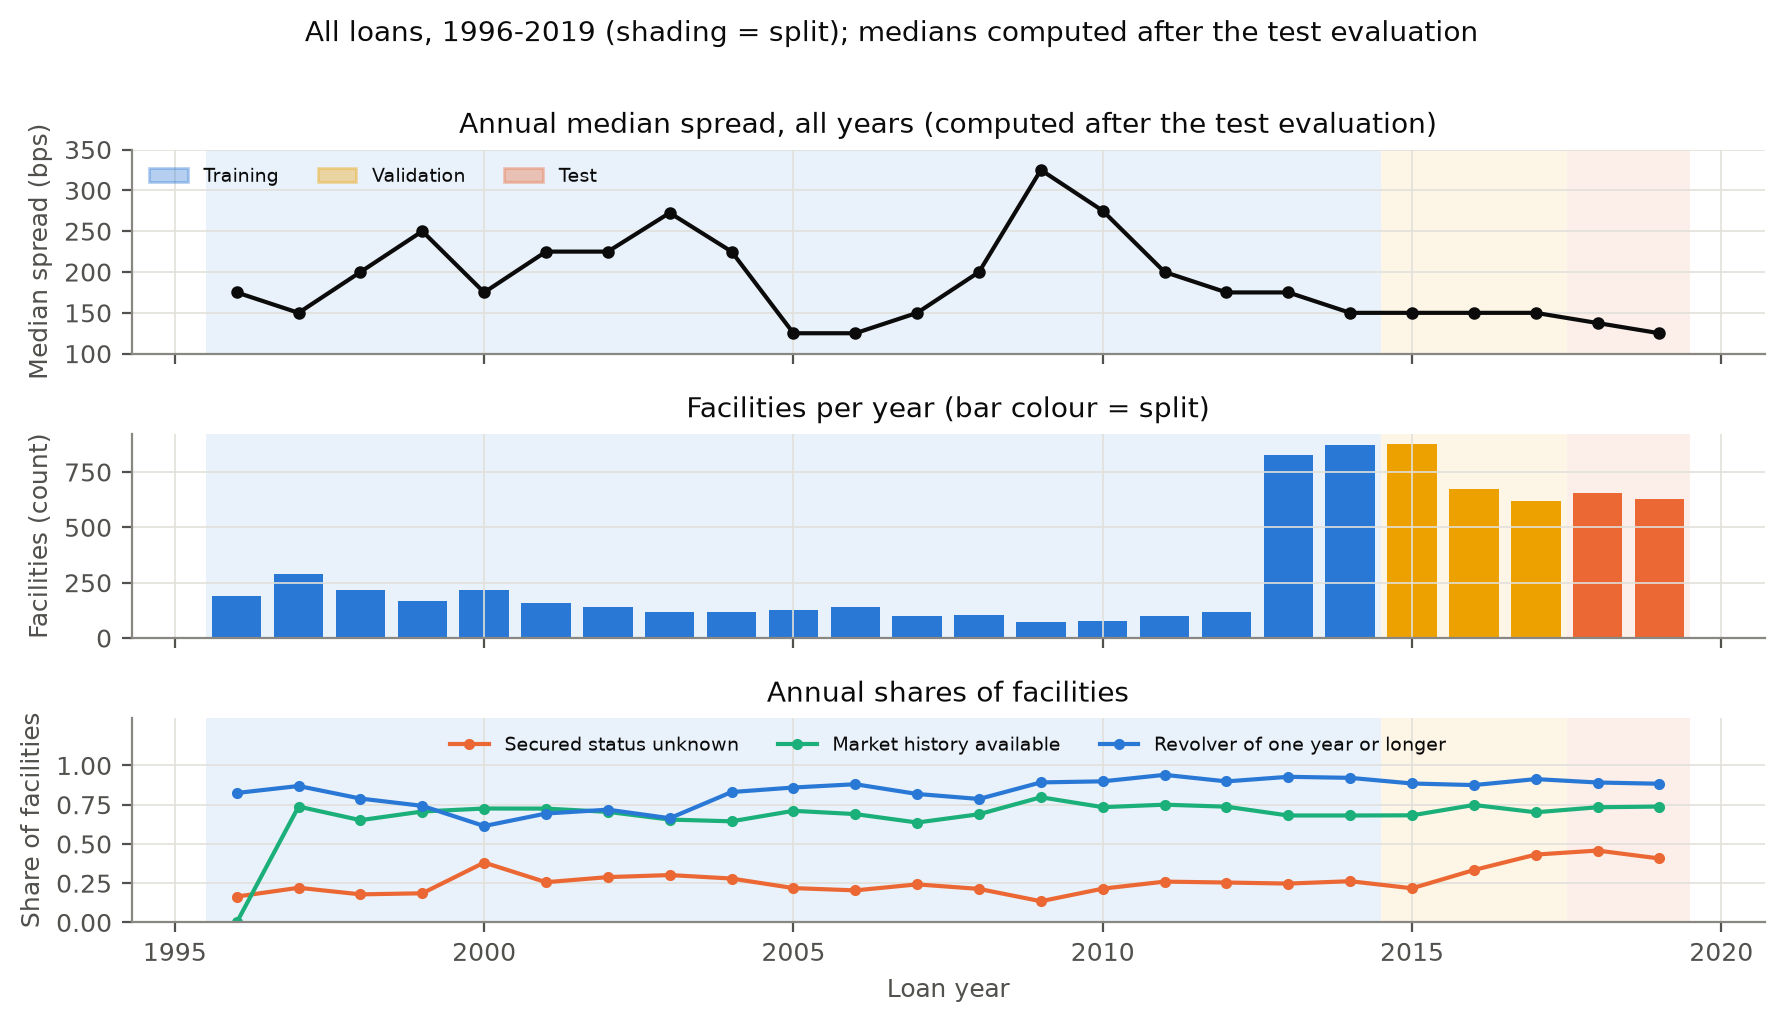
\includegraphics[width=0.93\textwidth]{sample_over_time.png}
\par\vspace{1pt}
\captionof{figure}{All facilities, 1996-2019 (7,605 facilities; shading marks the training, validation and test periods). Spreads in bps. The annual median spread uses the full period and was computed after the test evaluation; counts, shares and dates use all rows.}
\end{center}

% ======================================================================
% PAGE 3: model selection
% ======================================================================
\needspace{5\baselineskip}
\section*{Model selection (Section 3)}
\begin{figure}[!t]
\centering
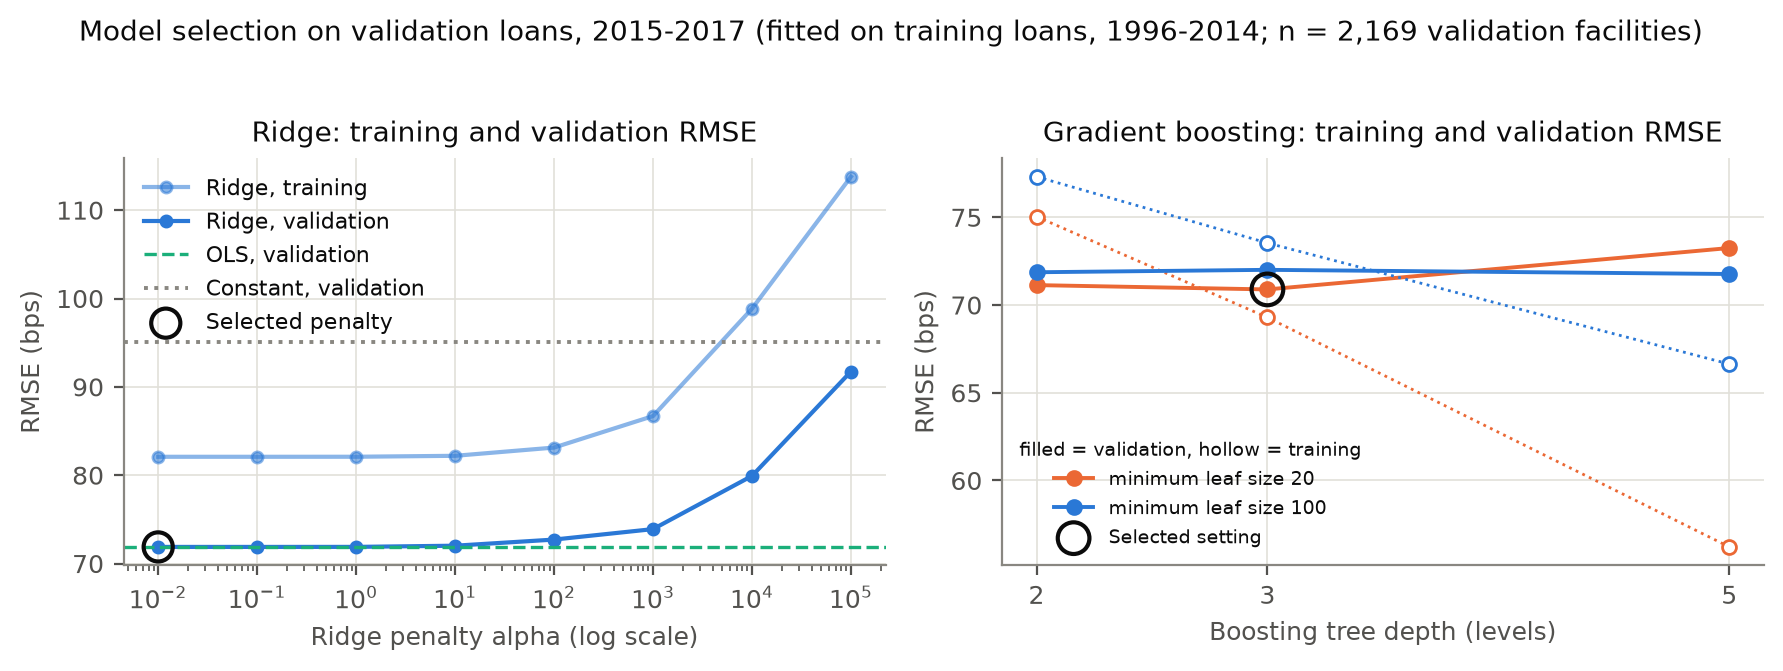
\includegraphics[width=\textwidth]{validation_selection.png}
\par\vspace{1pt}
\captionof{figure}{Selection on validation loans, 2015-2017 (2,169 facilities), with models fitted on training loans, 1996-2014 (4,157 facilities). RMSE in bps. Left: Ridge by penalty, with the OLS and constant benchmarks; right: gradient boosting by tree depth and minimum leaf size (filled: validation, hollow: training). Rings mark the selected settings.}
\end{figure}

\begin{itemize}
  \item \textbf{Against the benchmark.} On the validation sample (constant benchmark RMSE 95.1~bps), OLS, Ridge, and Gradient boosting have a clearly lower RMSE than the constant benchmark (71.9, 71.9, and 70.9~bps; borrower-clustered interval excludes zero).
  \item \textbf{Role of regularization.} The best validation RMSE came at the smallest penalty in the grid ($\alpha$ = 0.01), so regularization did not reduce validation RMSE, the selection criterion: Ridge ($\alpha$ = 0.01) and OLS are about equally accurate on the validation sample (RMSE 71.9 vs 71.9~bps, a difference of 0.0\%). Moderate shrinkage does lower validation MAE (from 47.5~bps for OLS to 45.0~bps at $\alpha$ = 1000) while raising RMSE (73.9~bps), i.e. it trades a few larger errors for many smaller ones. Shrinkage does work mechanically: the coefficient norm falls from 227.2 for OLS to 4.2 at the largest penalty, but validation RMSE then rises to 91.7~bps, close to the constant benchmark's 95.1~bps.
  \item \textbf{Does nonlinearity help?} Gradient boosting (depth 3, min leaf 20) and Ridge ($\alpha$ = 0.01) are about equally accurate on the validation sample (RMSE 70.9 vs 71.9~bps, a difference of 1.4\%). The same classification holds against OLS (RMSE 71.9~bps). Consistent with overfitting: the deepest configuration (depth 5, minimum leaf 20) has a lower training RMSE (56.2 against 69.3~bps) but a higher validation RMSE (73.3 against 70.9~bps); this validation difference has no bootstrap classification. Boosting's RMSE is more than 2\% below OLS in 2017 and within 2\% of OLS in 2015 and 2016. The selected boosting fit has training RMSE 69.3~bps against validation 70.9~bps (gap +1.6~bps).
  \item \textbf{What the blocks add.} Ridge on the loan and borrower blocks is more accurate than Ridge on the loan block alone on the validation sample (RMSE 72.3 vs 75.5~bps, 4.3\% lower; the borrower-clustered bootstrap 95\% interval for the difference, [$-$4.5, $-$2.0]~bps, excludes zero). Ridge on all four blocks and Ridge on the loan and borrower blocks are about equally accurate on the validation sample (RMSE 71.9 vs 72.3~bps, a difference of 0.5\%). Table~\ref{tab:blocks} gives the details; these are descriptive comparisons on validation loans, not tests.
\end{itemize}

\begin{center}
\small
\setlength{\tabcolsep}{4pt}
\begin{tabular}{@{}lcrrrll@{}}
\toprule
\textbf{Specification} & \textbf{Features (cols)} & \textbf{$\alpha$} & \textbf{Valid.\ RMSE} & \textbf{Valid.\ MAE} & \textbf{Change [95\% interval]} & \textbf{Classification} \\
\midrule
(a) Loan and industry & 6 (28) & 100 & 75.5 & 48.3 & -- & -- \\
(b) (a) + borrower financials & 15 (45) & 100 & 72.3 & 45.2 & $-$3.2 [$-$4.5, $-$2.0] & A clearly lower RMSE \\
(c) (b) + market, macro & 20 (51) & 0.01 & 71.9 & 47.5 & $-$0.4 [$-$2.2, +1.2] & about equal (within 2\%) \\
\bottomrule
\end{tabular}
\par\vspace{2pt}
\captionof{table}{Ridge on validation loans, 2015-2017 (2,169 facilities), fitted on training loans, 1996-2014, with the penalty re-tuned for each specification on the same candidate values. RMSE and MAE in bps. Change: RMSE of the specification minus RMSE of the row above, with the borrower-clustered bootstrap interval (2,000 resamples of whole borrowers); the interval is descriptive, not a test. In the classification, A is the larger specification.}
\label{tab:blocks}
\end{center}

% ======================================================================
% PAGE 4: test evaluation
% ======================================================================
\needspace{5\baselineskip}
\section*{Test evaluation (Section 4)}
\begin{center}
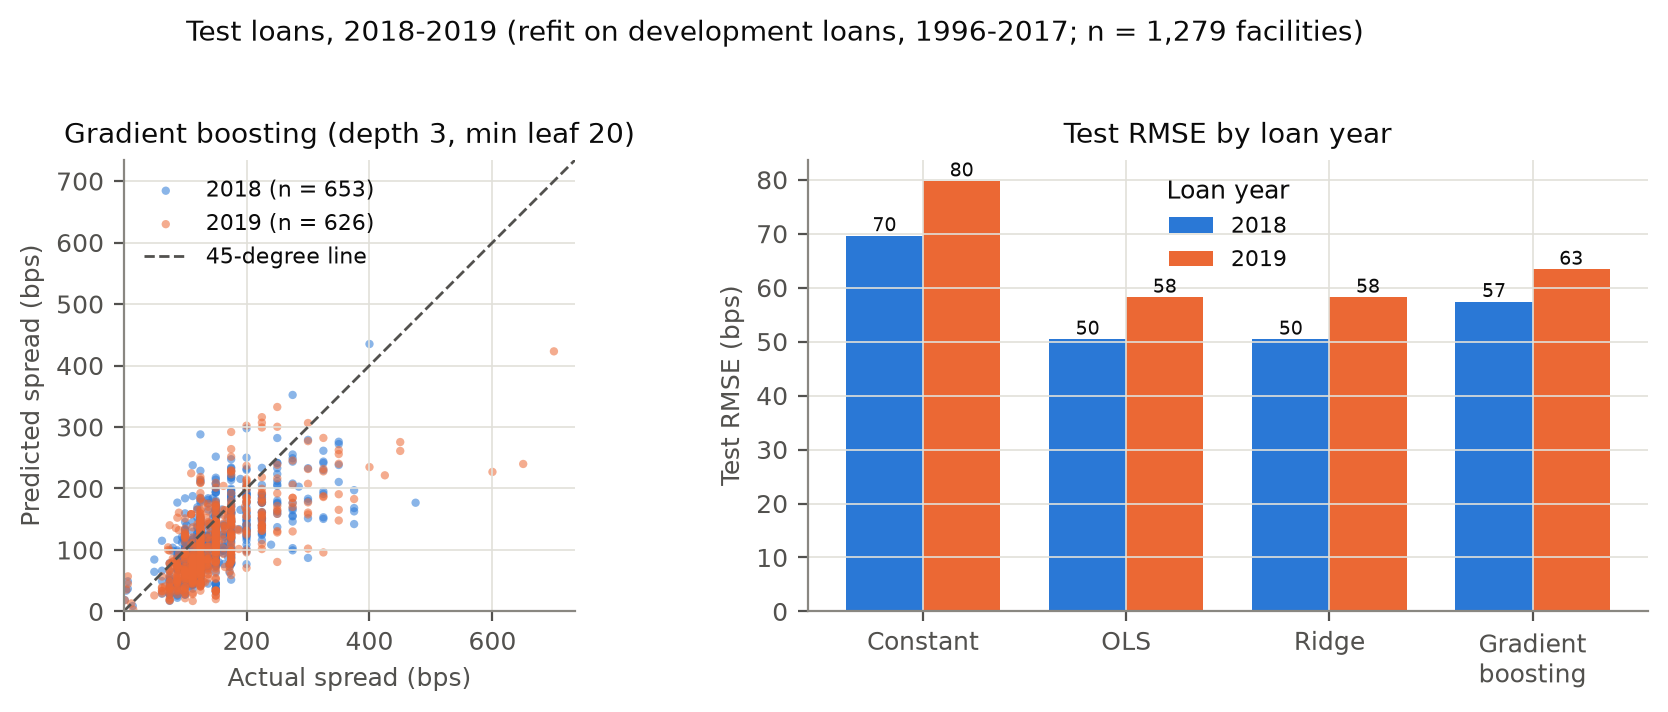
\includegraphics[width=0.68\textwidth]{test_actual_vs_predicted.png}
\par\vspace{1pt}
\captionof{figure}{Test loans, 2018-2019 (1,279 facilities); models refit on training plus validation loans. Spreads and RMSE in bps. Left: actual against predicted spread for the validation-selected preferred model, Gradient boosting (depth 3, min leaf 20). Right: test RMSE by loan year for the four model families.}
\end{center}

\begin{itemize}
  \item \textbf{Against the benchmark.} On the test sample (constant benchmark RMSE 74.7~bps), OLS, Ridge, and Gradient boosting have a clearly lower RMSE than the constant benchmark (54.4, 54.4, and 60.4~bps; borrower-clustered interval excludes zero).
  \item $R^2_{\mathrm{OOS}}$ against the train+validation mean (187.5~bps): OLS 0.471, Ridge 0.471, Gradient boosting 0.347, and the constant benchmark 0 by construction; a positive value means lower test squared error than that benchmark. It is not the usual $R^2$. The benchmark over-predicts the test loans by 38.4~bps on average (this level shift, its squared mean error, is 26.3\% of its test mean squared error). For the preferred model, $R^2_{\mathrm{OOS}}$ of 0.347 splits into 0.054 from a smaller level error than the benchmark and 0.293 from smaller errors around the mean, so most of it comes from smaller errors around the mean. For OLS and Ridge, which have the same split to three decimals, $R^2_{\mathrm{OOS}}$ of 0.471 splits into 0.195 from a smaller level error than the benchmark and 0.275 from smaller errors around the mean (the two parts add up to the total before rounding). As a diagnostic only, measured against the test-period mean (149.1~bps; not known in advance), the preferred model's value is 0.114.
  \item \textbf{Simple versus flexible models.} Gradient boosting (depth 3, min leaf 20) is substantially less accurate than OLS on the test sample (RMSE 60.4 vs 54.4~bps, 11.1\% higher; the borrower-clustered bootstrap 95\% interval for the difference, [4.0, 7.9]~bps, excludes zero). The same classification holds against Ridge (Ridge RMSE 54.4~bps). Ridge ($\alpha$ = 0.01) and OLS are about equally accurate on the test sample (RMSE 54.4 vs 54.4~bps, a difference of 0.0\%). A complex model need not beat a simpler one. The test gap to Ridge is mostly a difference in level: mean errors (actual minus predicted) are +34.2 and +19.5~bps, squared bias 1,170.7 and 380.4~bps$^2$, while the variance of the errors around their mean is 3.8\% lower for the preferred model (2,477.7 and 2,576.5~bps$^2$).
  \item \textbf{Test versus validation levels.} Test RMSEs are lower than validation RMSEs for every model, including the constant benchmark (preferred model 60.4~bps on test against 70.9~bps on validation; constant benchmark 74.7 against 95.1~bps). Lower test RMSEs are not evidence of stronger modeling. A possible explanation is composition: test spreads have a standard deviation of 64.2~bps against 91.4~bps in the validation sample, so less spread variation is left to predict.
  \item \textbf{By test year.} The preferred model's test RMSE is 57.4~bps in 2018 and 63.4~bps in 2019 (653 and 626 facilities), against 69.6 and 79.8~bps for the constant benchmark; relative to the benchmark the two years are similar ($R^2_{\mathrm{OOS}}$ 0.320 in 2018 and 0.368 in 2019); the higher absolute error goes with more dispersed 2019 spreads (standard deviation 58.9 and 69.3~bps).
  \item \textbf{Seen versus new borrowers.} The preferred model's RMSE is 67.7~bps on the 116 test loans to borrowers not seen in training or validation against 59.6~bps on the 1,163 loans to seen borrowers, 13.6\% higher for new borrowers (imprecise for the smaller new-borrower group), but the difference is not robust to resampling borrowers (new minus seen +8.1~bps, interval [$-$4.8, +21.7]~bps).
  \item \textbf{Large errors.} 28 test loans (2.2\%) have an absolute error above 141.8~bps (twice the preferred model's validation RMSE, frozen before the test targets were read). 27 of 28 (96.4\%) are under-predictions; the 1,251 other test facilities are mostly under-predicted too (79.5\%), so the sign is not specific to the large errors. Their mean actual spread is 373.2~bps against 144.1~bps for other loans. Compared with the rate among the other facilities, they more often have a purpose other than corporate purposes (8 observed against 4.4 expected) and a realized spread above the 90th percentile of training and validation spreads (16 observed against 0.2 expected); unknown secured status, missing market history, missing total assets, a loan type other than the main revolver, and a new borrower occur about as often as expected given 28 facilities. The realized-spread group is defined by the outcome and cannot be identified at pricing; on its 24 test loans above 325.0~bps the constant benchmark's RMSE is 246.1~bps against 203.3~bps for the preferred model. Whether these loans carry risk not captured by the 20 predictors is a hypothesis the data here cannot test.
  \item \textbf{Sample changes over time.} Against training loans, test loans have a lower mean spread (149.1~bps against 196.5~bps), less dispersed spreads (standard deviation 64.2 against 117.7~bps), larger borrowers (median \texttt{log\_assets} 8.694 against 6.782 ln USD millions), and a higher share of unknown secured status (43.3\% against 24.5\%). Whether these shifts change the model's accuracy relative to the benchmark cannot be tested with these data.
  \item \textbf{Supplementary log-target Ridge.} Converted back to bps with a smearing factor (1.085 at the refit): on validation, the log-target Ridge has a lower RMSE than Ridge with $\alpha$ = 0.01 (RMSE 70.2 vs 71.9~bps), but not robustly (the interval includes zero); on test, the log-target Ridge has a clearly lower RMSE than Ridge with $\alpha$ = 0.01 (RMSE 51.0 vs 54.4~bps; the bootstrap interval excludes zero), with test $R^2_{\mathrm{OOS}}$ 0.534, which splits into 0.225 from a smaller level error than the benchmark and 0.308 from smaller errors around the mean (the two parts add up to the total before rounding). It is not eligible to be the preferred model.
  \item \textbf{Dependence.} Facilities in one package and repeated loans to one borrower are dependent, so row-level differences are not independent evidence. The bootstrap resamples 885 test borrowers with all their facilities (2,000 draws, 95\% interval); it is descriptive, not a significance test, and ignores common time effects such as shared macroeconomic conditions.
\end{itemize}

% ======================================================================
% PAGE 5: interpretation, assessment and limitations
% ======================================================================
\needspace{5\baselineskip}
\section*{Interpretation and assessment (Section 5)}
\begin{figure}[!t]
\centering
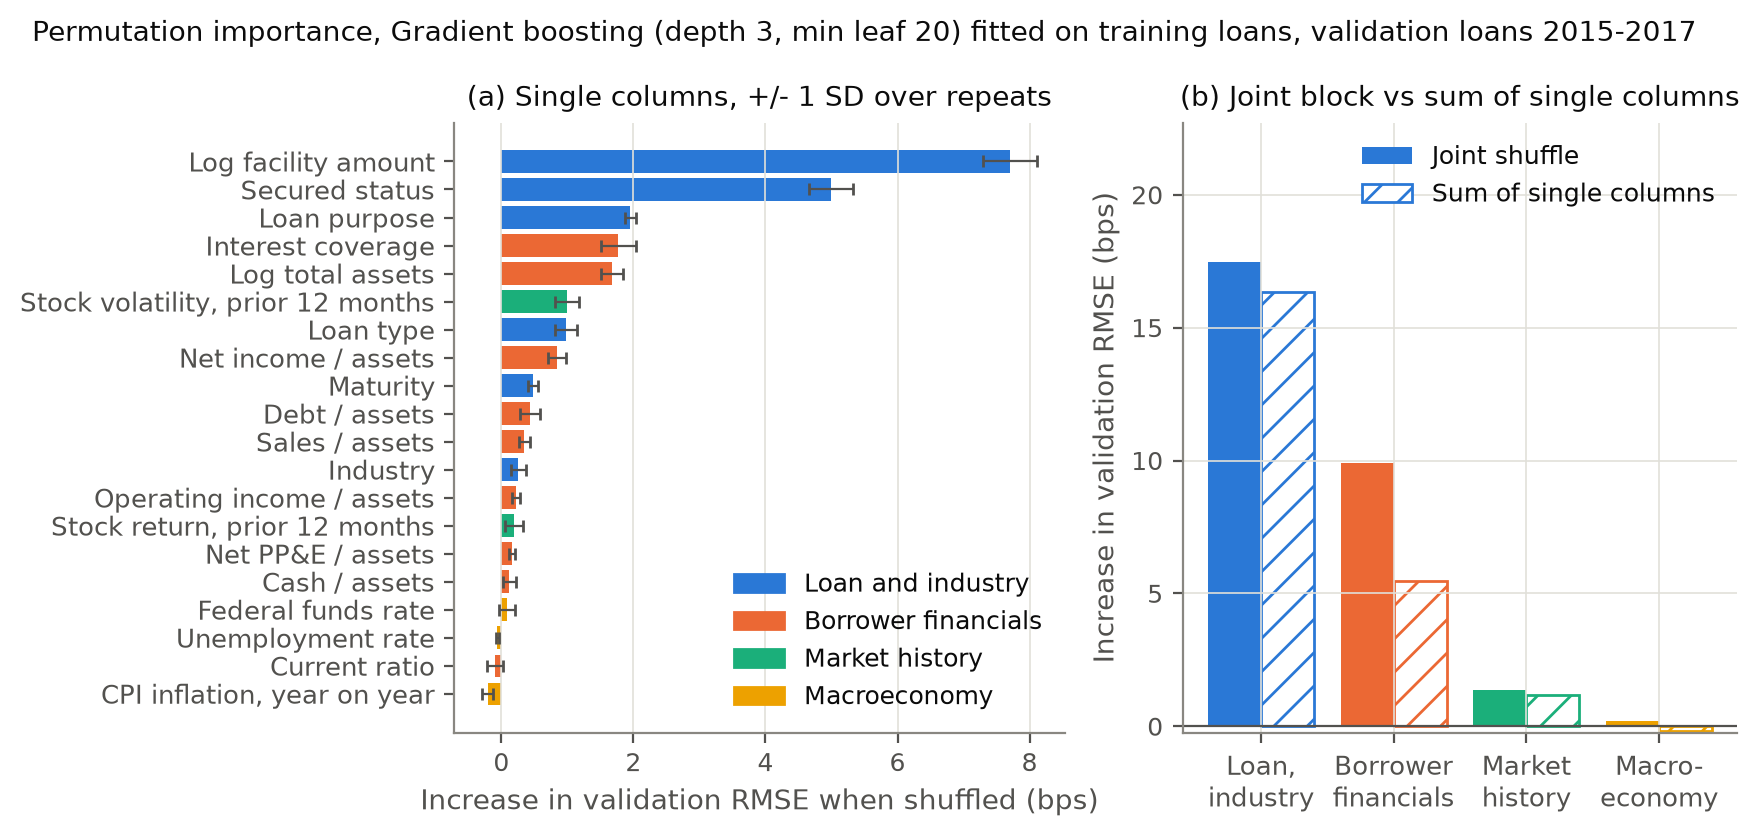
\includegraphics[width=0.64\textwidth]{permutation_importance.png}
\par\vspace{1pt}
\captionof{figure}{Permutation importance of the preferred model (fitted on training loans) on validation loans, 2015-2017 (2,169 facilities): RMSE increase (bps) when columns are shuffled (20 repeats; mean and one SD). Right: joint block shuffle against the sum of single columns.}
\end{figure}
\begin{figure}[!t]
\centering
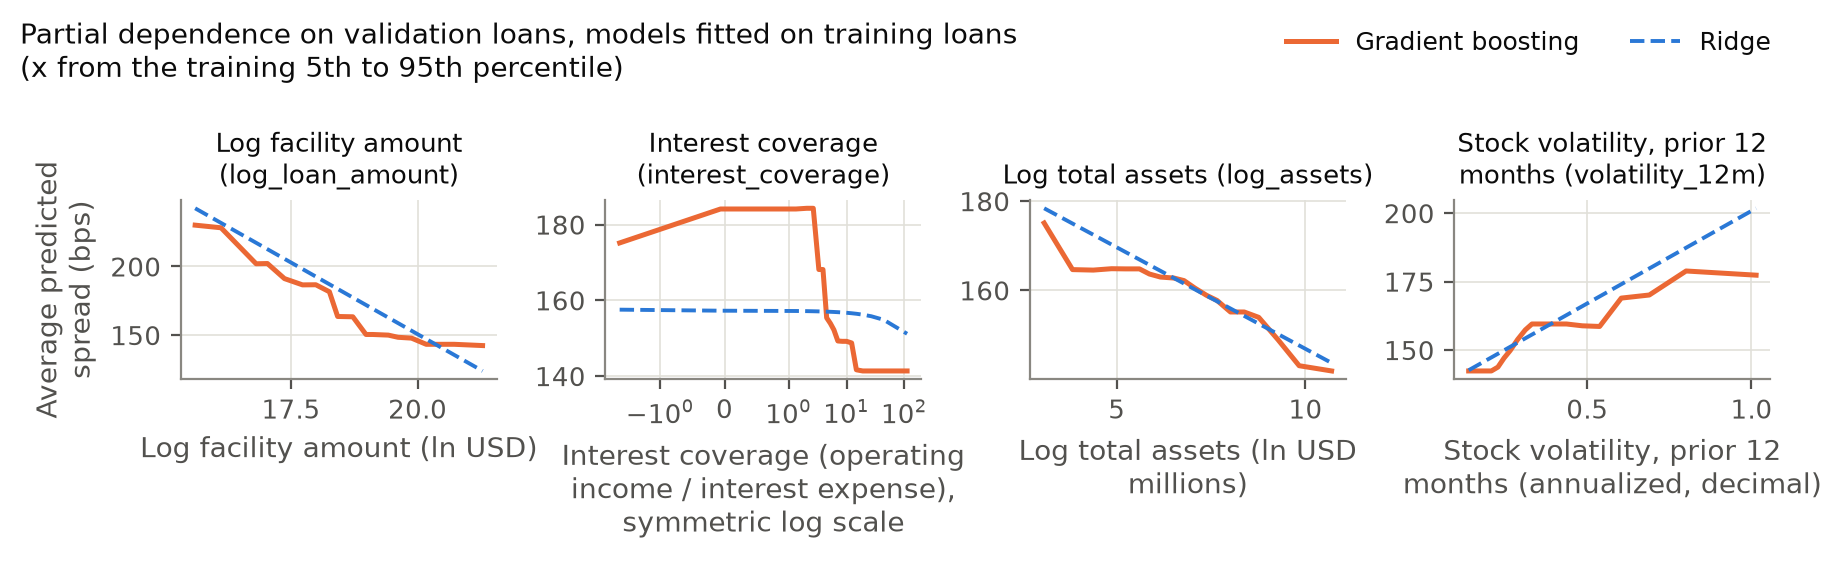
\includegraphics[width=0.72\textwidth]{partial_dependence.png}
\par\vspace{1pt}
\captionof{figure}{Partial dependence on validation loans for the four most important numeric features (each in its own units; average predicted spread in bps).}
\end{figure}

\begin{itemize}
  \item \textbf{Most important variables.} Shuffling a single column of the validation loans raises the preferred model's RMSE most for \mbox{\texttt{log\_loan\_amount}} (7.7), \mbox{\texttt{secured}} (5.0), \mbox{\texttt{loan\_purpose}} (1.9), \mbox{\texttt{interest\_coverage}} (1.8), and \mbox{\texttt{log\_assets}} (1.7), in bps against a baseline validation RMSE of 70.9~bps. The macroeconomy block has the smallest joint importance (0.2~bps).
  \item \textbf{Shared importance.} Joint block shuffle against the sum of single-column shuffles: the joint importance exceeds the sum of single-column importances by more than the repeat-to-repeat noise for borrower financials (9.9 vs 5.5~bps; difference 4.5~bps, computed before rounding, against a noise SD of 0.65~bps); joint and summed importances are within noise of each other for market history (+0.2~bps against a noise SD of 0.35~bps); the joint importance is close to the sum for loan and industry (exceeding it by 1.1~bps, more than the noise SD of 0.83~bps but less than 10\% of the sum); the comparison is not informative for macroeconomy (single-column sum $-$0.2~bps, not positive; joint importance 0.2~bps).
\end{itemize}
\needspace{8\baselineskip}
\begin{itemize}
  \item \textbf{Direction of relationships.} Partial dependence, the Ridge coefficient and the training quintile medians agree in sign for all four features. The preferred model's curve for \mbox{\texttt{interest\_coverage}} rises from 175.2~bps at the 5th percentile to 184.1~bps at the 10th before falling to 141.4~bps at the 95th. Sizes differ strongly from the Ridge comparison model for \mbox{\texttt{interest\_coverage}} ($-$42.8 against $-$2.4~bps, larger for the preferred model). In the preferred model, moving \texttt{log\_loan\_amount} from its training 10th to 90th percentile changes the average predicted spread by $-$84.9~bps (higher \texttt{log\_loan\_amount} goes with lower predicted spreads); the Ridge coefficient points the same way ($-$36.1~bps per SD); training quintile medians move by $-$150.0~bps from the lowest to the highest quintile (falling; 7.2\% of training loans with a \texttt{log\_loan\_amount} value have a value shared with loans in another quintile and tied loans are assigned to quintiles in file order, which follows the origination date). For \texttt{secured}, the average predicted spread is 172.0~bps if every validation loan is treated as secured, 36.2~bps lower if unsecured and 24.8~bps lower if status is unknown (differences computed before rounding). The preferred model has secured loans priced higher, which is consistent with the second channel (collateral requested from riskier borrowers) outweighing the first (lower loss given default); it does not measure the effect of collateral.
  \item \textbf{Importance is not direction or causality.} Permutation importance shows how much prediction suffers when a column is scrambled, not its sign, and correlated features can share importance (for example \mbox{\texttt{log\_loan\_amount}} and \mbox{\texttt{log\_assets}}, Spearman correlation 0.77). Loan size and secured status are set jointly with the spread, while borrower and market characteristics are observed, not assigned, and may move with unobserved credit quality (the data cannot test this), so these are predictive associations, not causal effects. This is not an automated lending decision.
\end{itemize}

\subsection*{Assessment and limitations}
\begin{itemize}
  \item \textbf{Where it adds value.} The preferred model adds value relative to the constant benchmark (test RMSE 60.4~bps against 74.7~bps; $R^2_{\mathrm{OOS}}$ 0.347, of which 0.054 from a smaller level error and 0.293 from smaller errors around the mean), with a bootstrap interval that excludes zero.
  \item \textbf{Where it is unreliable.} The preferred model under-predicts later loans in general: mean error +34.2~bps, 79.9\% of test facilities under-predicted, and the squared mean error is 32.1\% of its test mean squared error. Large errors: 27 of 28 (96.4\%) are under-predictions; the 1,251 other test facilities are mostly under-predicted too (79.5\%), so the sign is not specific to the large errors. Absolute errors are largest on loans whose realized spread turned out highest (above 325.0~bps): RMSE 203.3~bps on these 24 test loans against 54.1~bps on the other 1,255; the group is defined by the outcome, so it cannot be identified at pricing. Not listed as a weakness: borrowers not seen before (RMSE 67.7 vs 59.6~bps for 116 new and 1,163 seen borrowers' facilities, higher for new borrowers but not robust to resampling borrowers; imprecise). Model choice: it ranks 3 of 3 on test RMSE and the preferred model has a clearly higher RMSE than Ridge (RMSE 60.4 vs 54.4~bps; the bootstrap interval excludes zero); it is kept as required.
  \item \textbf{Information needed for real lending.} Credit ratings, market-implied credit spreads, covenant and collateral detail, separately reported fees, syndicate and relationship information, point-in-time filings, private-firm coverage and loan outcomes.
  \item \textbf{Limitations.} This is a retrospective pricing exercise, not a verified live underwriting backtest: the six-month accounting delay is an assumed availability proxy, and Compustat, FRED, links and industry codes are retrospective and may be revised. The sample is a selected linked sample; most test borrowers were seen before; market features are missing for 31.16\% of facilities, not at random; the evidence is one chronological split; and dependence within packages and borrowers limits row-level comparisons.
\end{itemize}

\end{document}
